\clearpage
\section{Figures moved from the main text}
\label{app:figs}
\begin{figure}[t]
\centering
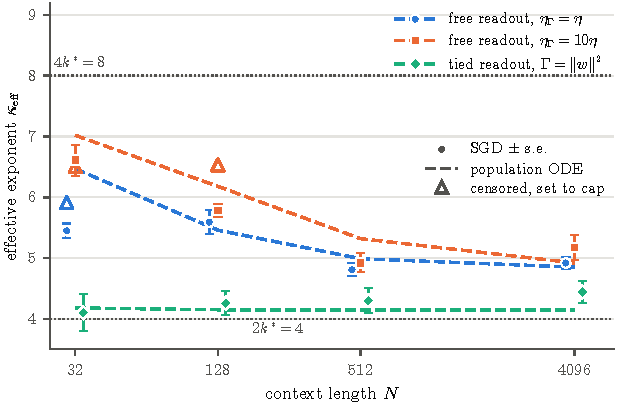
\includegraphics[width=.63\linewidth]{figs/fig_kappa.pdf}
\caption{Effective exponent of skill acquisition for $k^*=2$ at $d=32$: online SGD (points, $\pm$s.e.; triangles: censored runs
set to the step cap) against the parameter-free population ODE (dashed). The tied readout stays near $2k^*=4$ ($4.1$--$4.4$); the free readout
rises towards $4k^*=8$ as the context shortens.}
\label{fig:kappa}
\end{figure}

\begin{figure}[t]
\centering
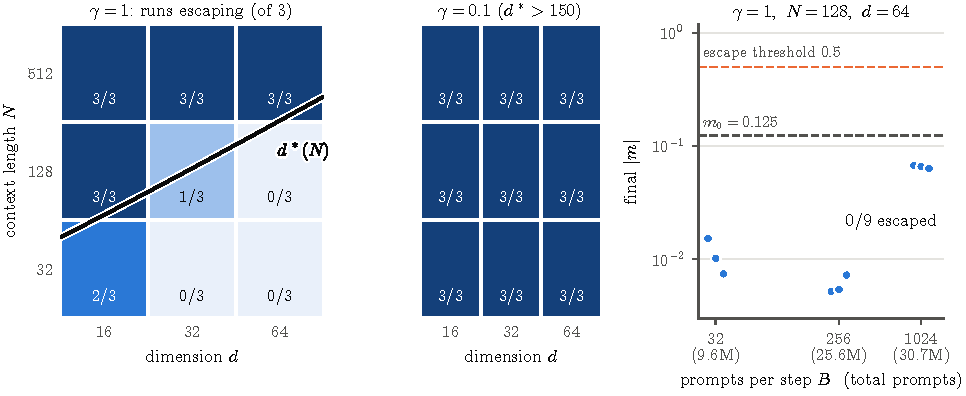
\includegraphics[width=\linewidth]{figs/fig_threshold.pdf}
\caption{Left: fraction of runs escaping $m_0=d^{-1/2}$ within $3\cdot10^5$ steps (fixed readout, 3 seeds per cell; curve: $d^*(N)$ of
Prop.~\ref{prop:repulsion}; for $\gamma=0.1$ the curve lies above the grid). Right: at $\gamma=1$, $N=128$, $d=64$ no run escapes for
$B\in\{32,256,1024\}$ prompts per step (total prompts $\times1$, $\times2.7$, $\times3.2$) and the final overlap falls \emph{below} $m_0$:
more prompts do not substitute for context length.}
\label{fig:threshold}
\end{figure}

\begin{figure}[t]
\centering
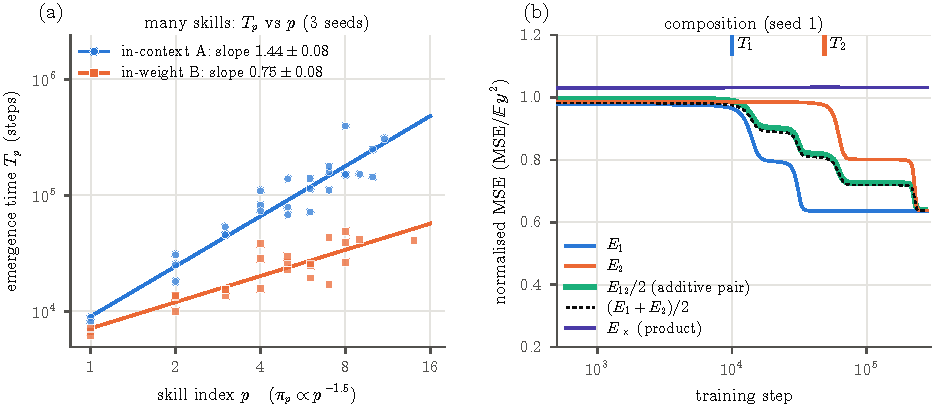
\includegraphics[width=\linewidth]{figs/fig_many.pdf}
\caption{(a) Emergence time (drop midpoint) of skill $p$ versus skill index for the in-context model (slope $1.44\pm0.08$), the
capacity-matched in-weight baseline (slope $0.75\pm0.08$) and the 2-homogeneous in-weight student (slope $0.75$--$0.89$), $\pi_p\propto p^{-1.5}$,
three seeds each; unlearned skills omitted.
(b) Composition (Exp.~3, one seed): normalised MSE on skill-1 prompts, skill-2 prompts, the additive pair (halved) and the product
pair; the dotted curve is half the sum of the single-skill losses and lies on the pair curve. Plateaus at $0.64$ are the fixed-readout
floor $(1-\Gamma n)^2$, not zero.}
\label{fig:many}
\end{figure}

\begin{figure}[t]
\centering
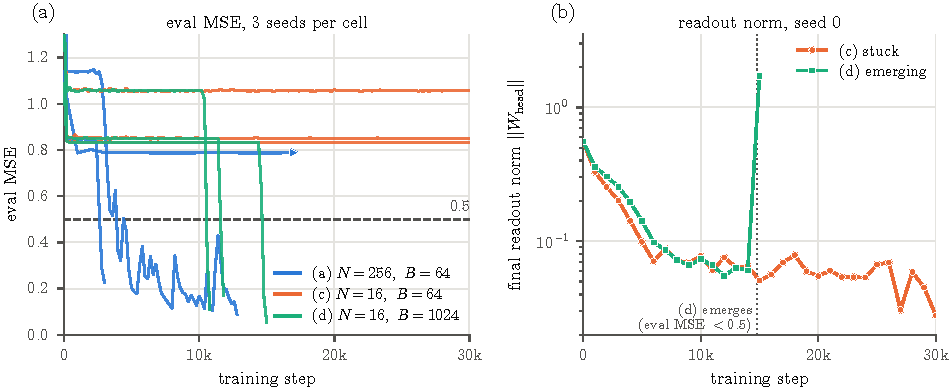
\includegraphics[width=\linewidth]{figs/fig_transformer.pdf}
\caption{Two-layer softmax transformer, $d=256$, MLP width 32, $k^*=2$. (a) Evaluation MSE for $N{=}256,B{=}64$; $N{=}16,B{=}64$; and
$N{=}16,B{=}1024$ (same tokens per step as the first), three seeds each; one $N{=}256$ seed was censored at $17$k steps on the plateau.
(b) Norm of the final readout for one stuck run ($N{=}16,B{=}64$) and one emerging run ($N{=}16,B{=}1024$, same seed): the norm
collapses while the skill is unlearned; the regrowth at emergence is a single logged point (norms logged every $1000$ steps).}
\label{fig:transformer}
\end{figure}
